El valor de las celdas para la colocación del extractor de minerales se realiza calculando la distancia de dicha casilla respecto al centro.
El valor de la casilla será el inverso de la distancia, de esta forma las casillas más cercanas al centro tendrán más valor.

% Elimine los símbolos de tanto por ciento para descomentar las siguientes instrucciones e incluir una imagen en su respuesta. La mejor ubicación de la imagen será determinada por el compilador de Latex. No tiene por qué situarse a continuación en el fichero en formato pdf resultante.
\begin{figure}
\centering
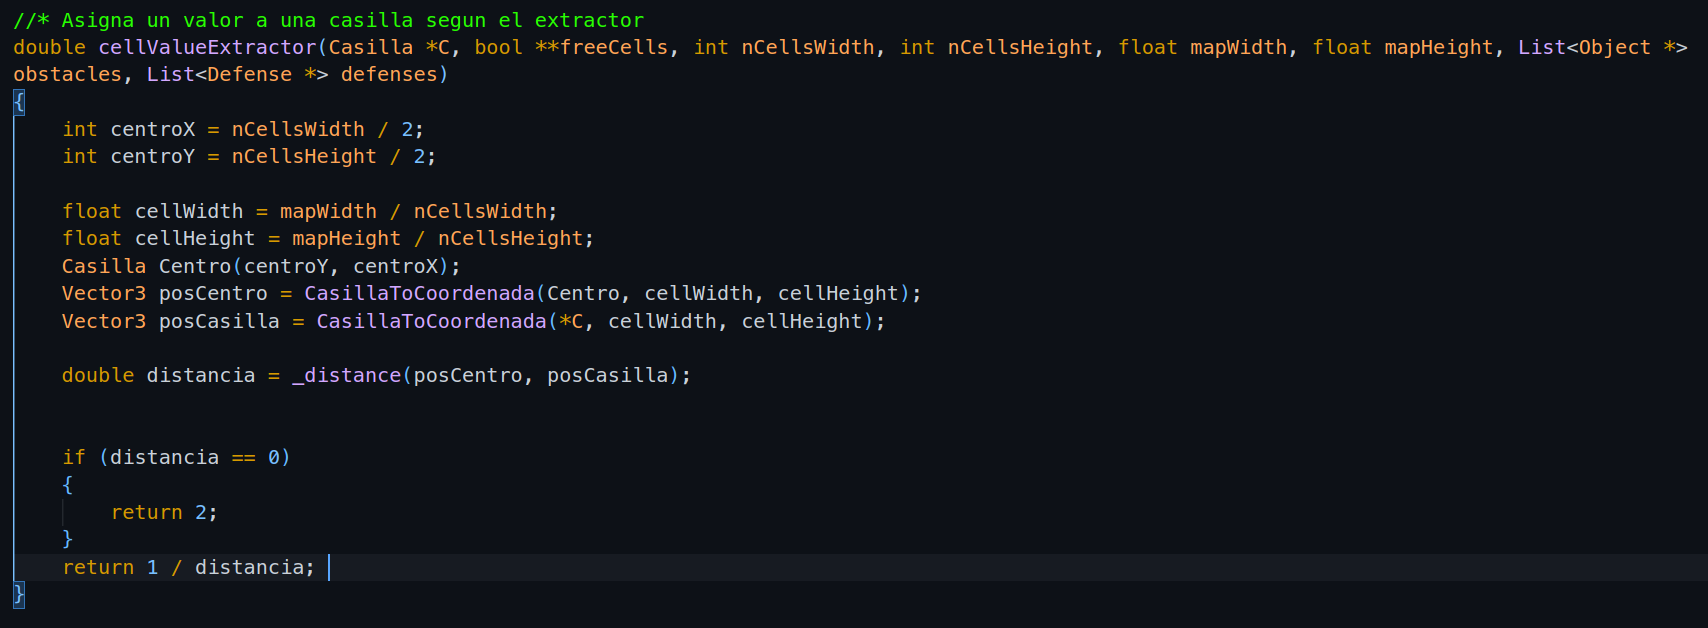
\includegraphics[width=0.7\linewidth]{./CellValueExtractor.png} % no es necesario especificar la extensión del archivo que contiene la imagen
\caption{Estrategia devoradora para la mina}
\label{fig:defenseValueCellsHead}
\end{figure}